% Created 2013-08-12 Mon 20:12
\documentclass[11pt]{article}
\usepackage[utf8]{inputenc}
\usepackage[T1]{fontenc}
\usepackage{fixltx2e}
\usepackage{graphicx}
\usepackage{longtable}
\usepackage{float}
\usepackage{wrapfig}
\usepackage[normalem]{ulem}
\usepackage{textcomp}
\usepackage{marvosym}
\usepackage{wasysym}
\usepackage{latexsym}
\usepackage{amssymb}
\usepackage{amstext}
\usepackage{hyperref}
\tolerance=1000
\date{\today}
\title{workflow}
\hypersetup{
  pdfkeywords={},
  pdfsubject={},
  pdfcreator={<a href="http://www.gnu.org/software/emacs/">Emacs</a> 24.2.1 (<a href="http://orgmode.org">Org</a> mode 8.0.6)}}
\begin{document}

\maketitle
\tableofcontents


\section{Workflows}
\label{sec-1}

\subsection{Review Workflow}
\label{sec-1-1}

\subsubsection{Review Queue}
\label{sec-1-1-1}
View the list of reviews you need to do. Click on reviews to do start your review, or delete a review.

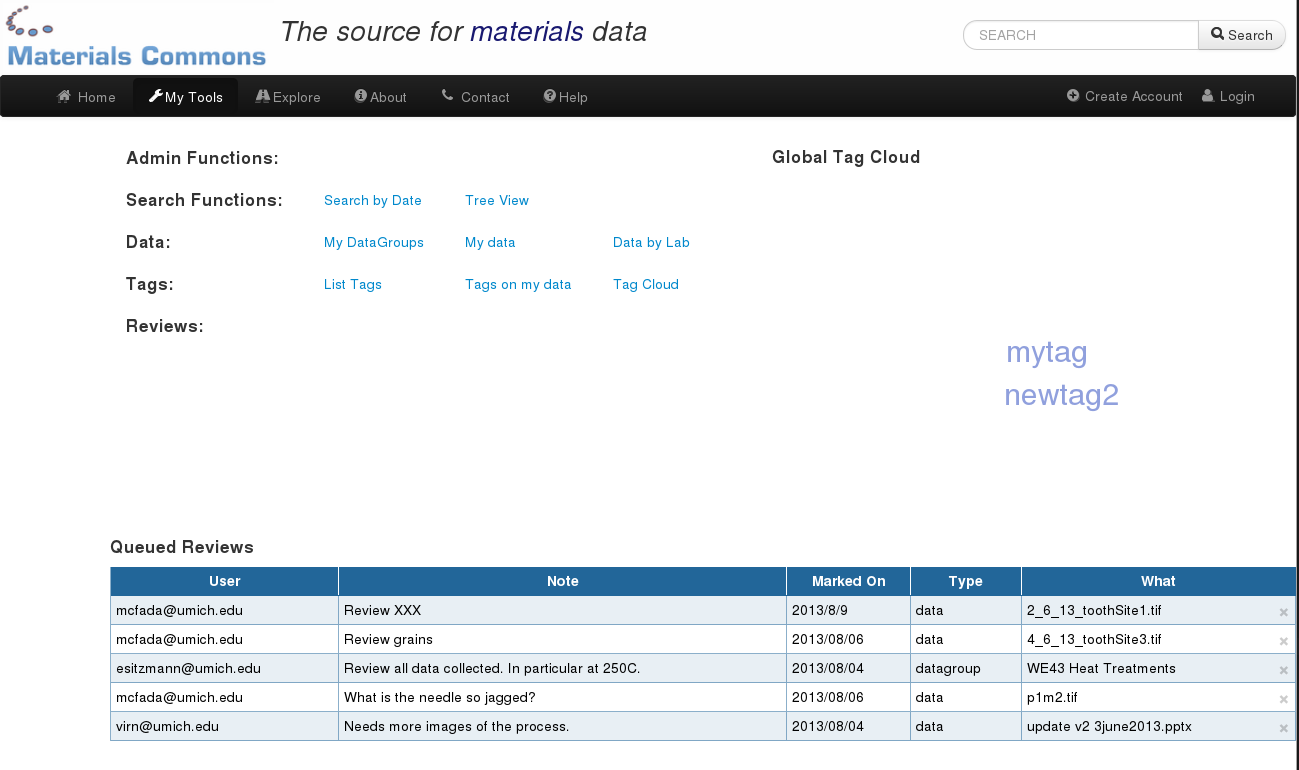
\includegraphics[width=.9\linewidth]{ReviewQueue.png}

\subsubsection{Data Review}
\label{sec-1-1-2}
View the list of reviews for a data item. Request reviews, or mark an item for future followup.

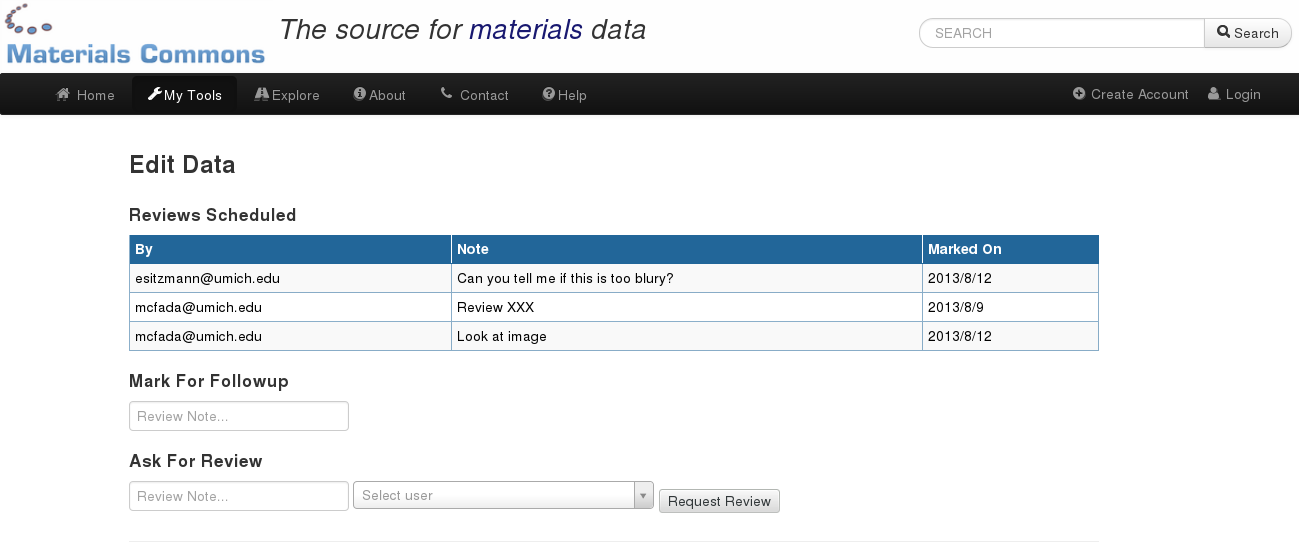
\includegraphics[width=.9\linewidth]{DataReview.png}
\subsection{Upload/Download Workflow}
\label{sec-1-2}
There will be two methods to upload/download files from the website. If a user installs
our send$_{\text{file}}$ package they will be able to queue their requests. The advantage to using
the send$_{\text{file}}$ package is that uploads and downloads can be done in the background. The
transfers will automatically restart if they are interrupted.

If a user doesn't have this package installed then they can choose to upload/download
files directly from the website. The download will take place through the browser and
the user will have to wait while it completes.

\subsubsection{Upload/Download Queue}
\label{sec-1-2-1}
View the list of queued upload/download requests and their current status.

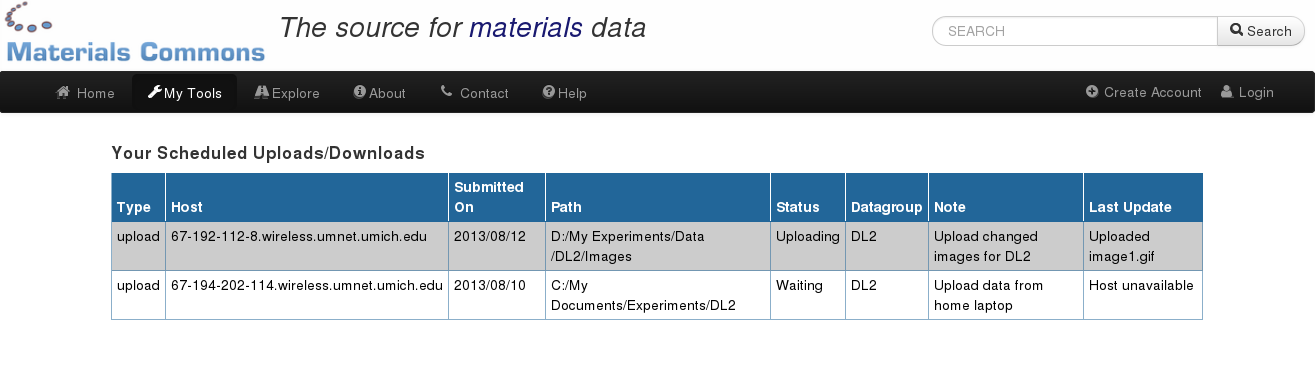
\includegraphics[width=.9\linewidth]{ScheduledUploadsDownloads.png}
\subsubsection{Upload Files}
\label{sec-1-2-2}
Choose files to upload and the datagroup to upload them to. All files go to the
same datagroup.

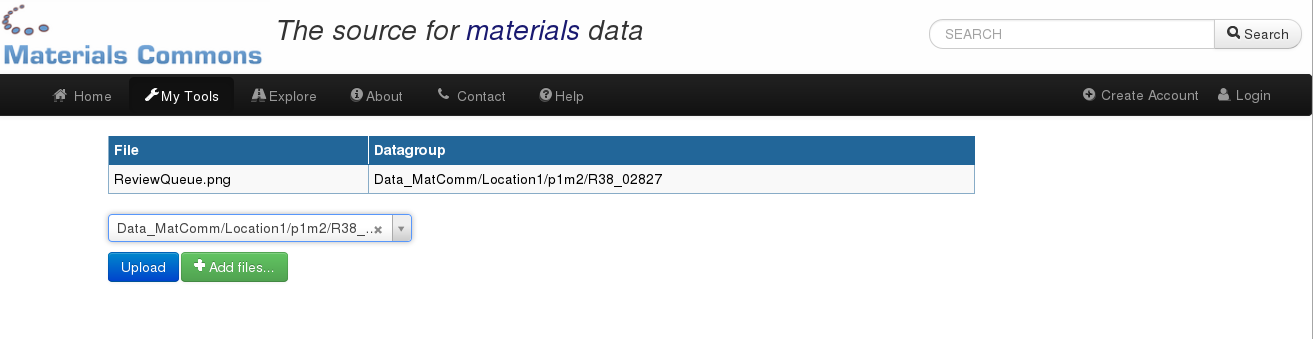
\includegraphics[width=.9\linewidth]{UploadFile.png}
\subsubsection{Upload Directories}
\label{sec-1-2-3}
Choose directories to upload and the datagroup to upload them to. All directories
go to the same datagroup.

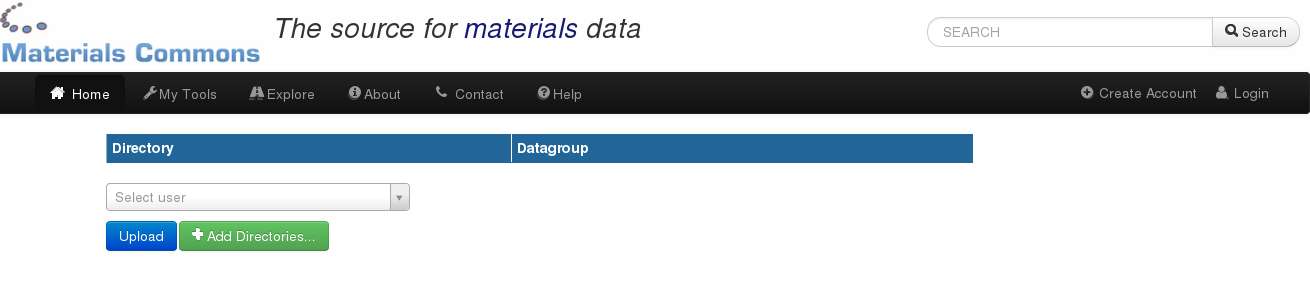
\includegraphics[width=.9\linewidth]{UploadDirectories.png}
% <a href="http://www.gnu.org/software/emacs/">Emacs</a> 24.2.1 (<a href="http://orgmode.org">Org</a> mode 8.0.6)
\end{document}
